% Online appendix for the LinePilot Digitizer manuscript.
\documentclass{article}
\usepackage[T1]{fontenc}
\usepackage{spconf,amsmath,amssymb,graphicx,booktabs,hyperref,array}
\usepackage[font=small]{caption}
\hypersetup{hidelinks}

\title{Online Appendix and Supplementary Materials for\\LinePilot Digitizer: Line-Plot Recovery with Manual and Automatic Calibration}
\name{\shortstack{Fengbo Ma\textsuperscript{1}, Rayan Akhtar\textsuperscript{1}, Aakash H. Joshi\textsuperscript{2}, Xiaoting Li\textsuperscript{1} \\
Haijian Sun\textsuperscript{1}, Yiping Zhao\textsuperscript{1}, Zhen Xiang\textsuperscript{1}, Xianyan Chen\textsuperscript{1}}}
\address{\textsuperscript{1}University of Georgia \qquad \textsuperscript{2}University of Pennsylvania}

\begin{document}
\maketitle

\tableofcontents

\section{Representative Digitization Example}
\label{sec:example}

Figure~\ref{fig:complete-example} expands the representative case summarized in the main manuscript. The example is an overlapping two-line plot rendered with Altair. Among the automatic pipelines, ChartOCR and LineEX produce no output, whereas LinePilot (OCR) reconstructs both series. Among the human-guided tools, PlotDigitizer Pro, WebPlotDigitizer, LinePilot (standard), and LinePilot (enhanced) recover both series, while Engauge Digitizer recovers only the blue series. The example illustrates three distinct evaluation outcomes: complete failure to return data, incomplete series recovery, and successful recovery with different levels of curve fidelity. It is intended as a qualitative case study; the aggregate conclusions are determined from DigitizerBench-Full and DigitizerBench-Lite rather than from this single image.

\begin{figure*}[t]
    \centering
    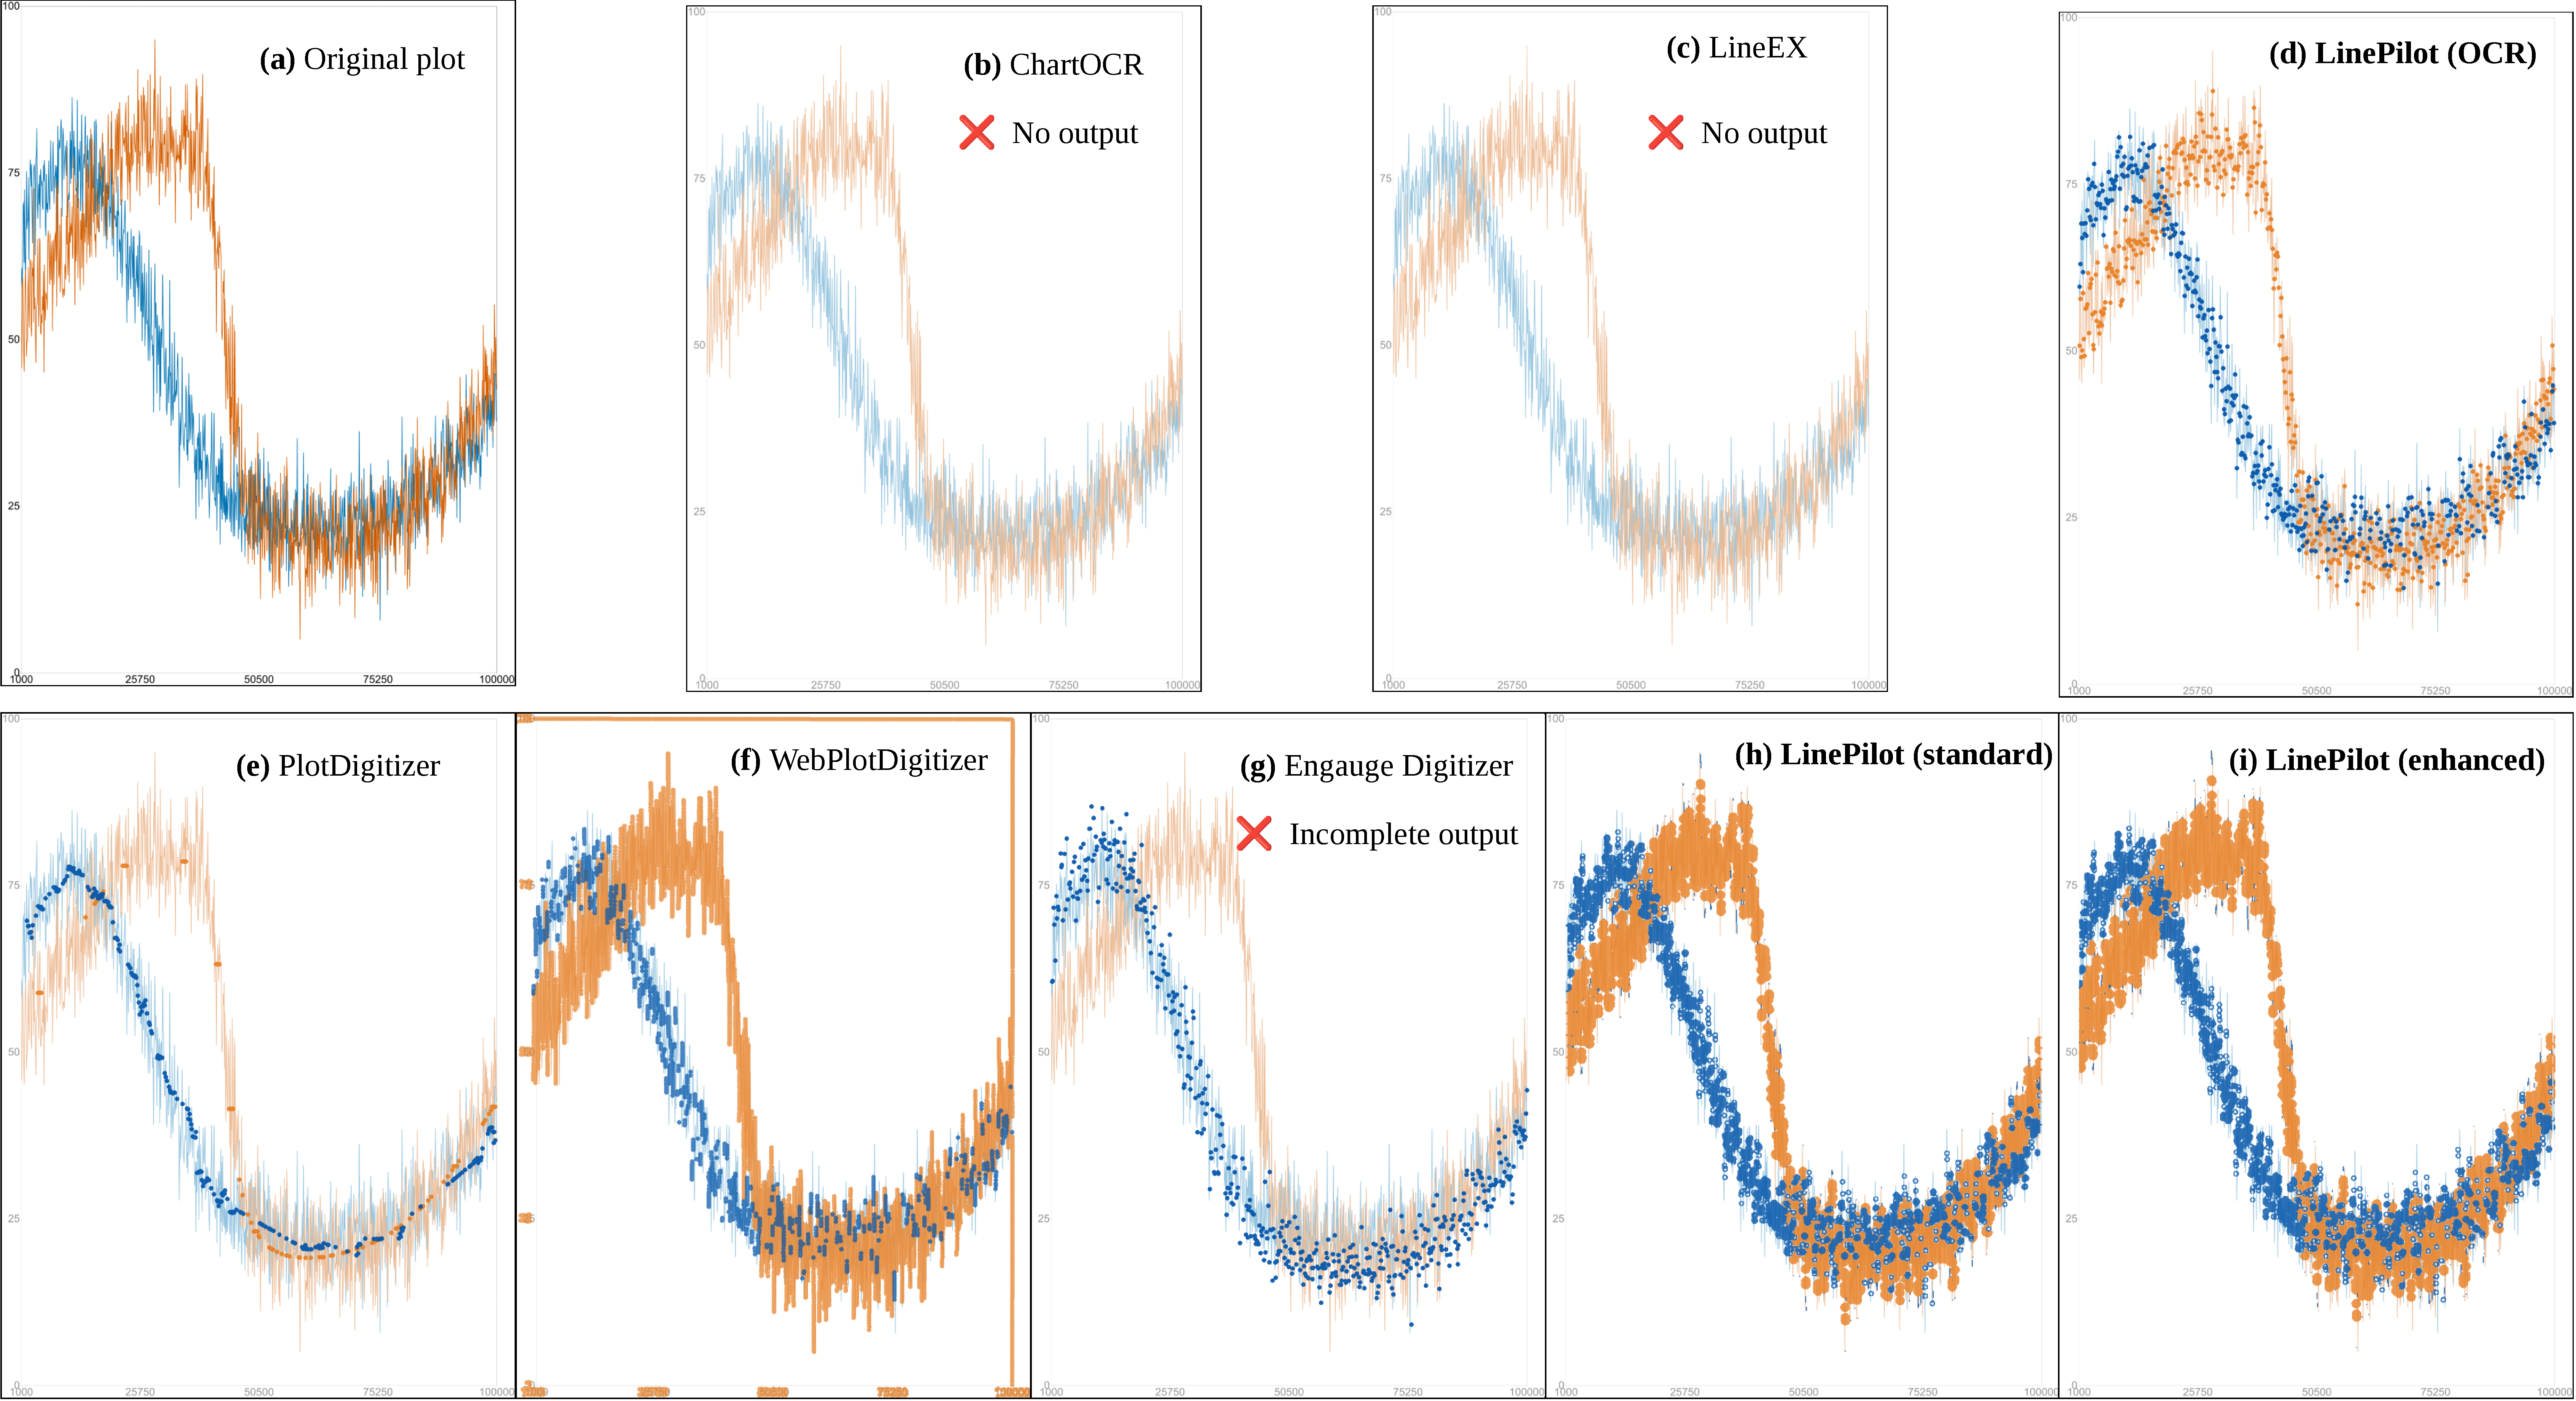
\includegraphics[width=0.96\textwidth]{figures/digitization-example.pdf}
    \caption{Digitization results for the \texttt{D0001-overlapping-altair} example from DigitizerBench. (a) Original plot. Automatic results: (b) ChartOCR~\cite{luo2021chartocr}, (c) LineEX~\cite{shivasankaran2023lineex}, and (d) LinePilot (OCR). Human-guided results: (e) PlotDigitizer Pro~\cite{plotdigitizer}, (f) WebPlotDigitizer~\cite{rohatgi_webplotdigitizer}, (g) Engauge Digitizer~\cite{mitchell_engauge}, (h) LinePilot (standard), and (i) LinePilot (enhanced). ChartOCR and LineEX produce no output, while Engauge Digitizer recovers only the blue series.}
    \label{fig:complete-example}
\end{figure*}

\section{DigitizerBench Construction Details}
\label{sec:construction}

DigitizerBench is designed to measure complete digitization performance under controlled signal, rendering, and plot-structure variation. The benchmark varies eight signal factors and ten rendering factors at five levels, together with plot type, line count, and renderer. The signal factors cover baseline behavior, extrema structure, feature shape, asymmetry, and numerical signal noise. The rendering factors cover line thickness and color, raster resolution, blur, physical figure dimensions, tick-label size and density, and numerical axis ranges. The three plot types are single-line, overlapping multiline, and vertically stacked multiline plots; the renderers are Matplotlib, Plotly, and Altair.

Four complementary strength-3 $\mathrm{OA}(625,19,5,3)$ panels~\cite{hedayat1999orthogonal} provide a 2,500-image orthogonal-array core. Within each panel, every combination of levels across any three design columns is balanced. This structure supports estimation of main effects with substantially fewer images than the exhaustive five-level factorial design, while the panel and generation block are retained as nuisance terms in the analysis.

Each numerical trace is generated independently from a baseline and a constrained sequence of peaks and valleys, then combined with independently generated Gaussian signal noise. Multiline traces do not share a latent curve. Overlapping plots place the completed traces on common axes without forcing intersections. Stacked plots add only the vertical offsets required to prevent intersections. A single positive affine mapping is then applied jointly to all traces in an image, preserving their relative shapes and noise levels. Exact numerical curves and tick coordinates are retained as ground truth, while digitizers receive only the rendered images.

All three renderers consume the same numerical plot specification and axis settings. Images use linear axes, solid lines, a white background, and no markers, legends, or grids. Renderer-specific width units are converted to target the assigned final-image line thickness, and blur is applied only after native image export. These controls distinguish the tested rendering effects from unintended changes to the numerical signal.

An outcome-independent constrained selection identifies 60 core configurations balanced across panels, plot types, renderers, and colors. Each selected configuration is rendered under all nine plot-type--renderer combinations. Because one combination is already present in the orthogonal-array core, this matched expansion adds 480 images to the 2,500-image core. DigitizerBench-Full therefore contains 2,980 images. The 60 original selected core images form DigitizerBench-Lite, and the complete nine-version expansion forms a 540-image matched bridge subset within DigitizerBench-Full. The bridge supports paired renderer and plot-type comparisons without treating the matched versions as independent configurations.

Reproducibility information includes the master seed, assigned factor levels, orthogonal-array panels, trace-generation rules, bridge membership, renderer versions, image specifications, and exact numerical and tick ground truth. The benchmark is constructed before digitizer evaluation, and neither bridge membership nor DigitizerBench-Lite membership uses digitizer outcomes.

\begin{table*}[t]
\centering\small
\caption{Summary of the DigitizerBench design.}
\label{tab:design-summary}
\setlength{\tabcolsep}{5pt}
\begin{tabular}{@{}p{0.19\textwidth}p{0.53\textwidth}p{0.19\textwidth}@{}}
\toprule
Component & Controlled variation & Design role \\
\midrule
Signal & Baseline family and magnitude; extrema count and prominence; feature width, sharpness, and asymmetry; signal noise & Five levels per factor in the orthogonal-array core \\
Rendering & Line thickness and color; DPI; blur; figure width and aspect ratio; tick-label size and count; x- and y-axis ranges & Five levels per factor in the orthogonal-array core \\
Plot structure & Single, overlapping, and stacked plots; one, two, three, or five lines as applicable & Balanced core allocation and matched bridge comparisons \\
Renderer & Matplotlib, Plotly, and Altair & Balanced core allocation and matched bridge comparisons \\
DigitizerBench-Full & 2,500 orthogonal-array core images plus 480 bridge images & Automatic evaluation and main-effects analysis \\
DigitizerBench-Lite & 60 outcome-independent core images & Human-guided evaluation on identical images \\
\bottomrule
\end{tabular}
\end{table*}

\section{Automatic Digitization: Effects of Benchmark Factors}
\label{sec:automatic-factors}

The automatic analysis uses the existing image-level failure-penalized capped normalized root-mean-square error (FPC-NRMSE) for LinePilot (OCR) on all 2,980 DigitizerBench-Full images. A main-effects analysis of variance includes panel, generation block, and image role as nuisance terms; conditional factors use their active populations. Adjusted sums of squares describe relative effect magnitude. Six prespecified two-factor interactions are examined in separate exploratory models by adding each interaction to the main-effects model. The reported $p$ values are unadjusted, and clustering by base image provides a sensitivity analysis for the repeated bridge renderings.

Figure width and DPI have the largest contributions to automatic performance, followed by renderer. Axis ranges, tick density, plot type, and blur have smaller significant effects. Signal noise and most curve-shape factors are not significant, showing that image presentation has a larger practical influence than signal complexity.

The response profiles clarify the practical scale of the largest effects. Adjusted mean FPC-NRMSE decreases from 0.930 for two-inch figures and 0.774 for three-inch figures to 0.530 at six inches and 0.480 at eight inches. For DPI, the adjusted mean decreases from 0.885 at 72 DPI and 0.774 at 100 DPI to 0.611 at 150 DPI; the 300- and 600-DPI levels are similar overall at 0.536 and 0.562. Thus, higher DPI alone does not compensate for an extremely narrow figure.

Two of the six prespecified interactions are significant. The width--DPI interaction confirms that physical size and raster resolution matter jointly: at 72 DPI, observed mean FPC-NRMSE remains between 0.84 and 1.00 across all widths, while two-inch figures remain poor at every DPI. The renderer--DPI interaction shows that Matplotlib and Plotly continue improving or remain stable at high DPI, whereas Altair improves through 300 DPI and worsens at 600 DPI in this benchmark. The remaining tested interactions are not significant.

Tick crowding and blur show smaller but interpretable trends. Five ticks per axis performs best among the tested levels, whereas degradation becomes clear at nine ticks and is strongest at eleven ticks. Results are similar from zero to 0.5 pixels of blur, with clearer degradation at 0.75 and 1.0 pixels. Although structural extrema count and prominence are statistically significant, each accounts for less than 0.5\% of adjusted variation and should not be described as a primary failure threshold. Overall, the automatic analysis shows that image presentation has a larger practical influence than signal complexity.

Because FPC-NRMSE is bounded and contains many unit-penalty outcomes, the ANOVA is an approximate large-sample analysis. The repeated bridge renderings are included in DigitizerBench-Full, and the base-image clustered sensitivity analysis is used to evaluate the effect of that dependence. These results describe the tested benchmark levels and do not establish universal thresholds outside those ranges.

\section{Human-Guided Digitization: Performance and Factor Effects}
\label{sec:human-factors}

The human-guided analysis evaluates LinePilot (standard) and LinePilot (enhanced) on the same 60 DigitizerBench-Lite images. The primary comparison is paired by image. In agreement with the main manuscript, LinePilot (enhanced) has the lower observed mean FPC-NRMSE (0.081 versus 0.101), 100\% output success, 93.3\% trusted usability, and the highest digitized-point density. LinePilot (standard) also has 100\% output success and 91.7\% trusted usability (Table~\ref{tab:human-summary}).

\begin{table}[t]
\centering\small
\caption{Human-guided LinePilot performance on DigitizerBench-Lite.}
\label{tab:human-summary}
\setlength{\tabcolsep}{3pt}
\begin{tabular}{@{}lrrrr@{}}
\toprule
Method & FPC-NRMSE & OS (\%) & TU (\%) & DPPL \\
\midrule
LinePilot (standard) & 0.101 & 100.0 & 91.7 & 1024.8 \\
LinePilot (enhanced) & \textbf{0.081} & 100.0 & \textbf{93.3} & \textbf{1026.5} \\
\bottomrule
\end{tabular}
\end{table}

The paired method effect is not statistically significant ($p=0.2362$). The defensible interpretation is therefore that LinePilot (enhanced) improves the observed mean and operational metrics, while this 60-image paired study does not establish a nonzero overall method effect.

DigitizerBench-Lite has only 60 independent image-level units and is not the full orthogonal design. Physical factors are therefore screened one at a time using the mean response of the two LinePilot modes, with adjustment only for plot type and renderer. These screens are exploratory associations rather than independent causal effects.

Line thickness shows the strongest association with human-guided performance and is the only physical factor reaching significance in the marginal screens ($p=0.0043$). One-pixel curves perform poorly, while performance stabilizes across three to five pixels. The effect applies to both LinePilot (standard) and LinePilot (enhanced).

The contrast with the automatic analysis suggests that human judgment can compensate for lower DPI through more reliable tick reading and reconstruction, whereas a very thin stroke can provide too little consistent color evidence for line selection and tracing.

In summary, LinePilot (enhanced) provides the best observed human-guided performance, but curve thinness---not the overall difference between the two clicking modes---is the strongest supported practical risk in DigitizerBench-Lite. DigitizerBench-Full should be used for independent system-factor attribution, while DigitizerBench-Lite supports the paired comparison of the two human-guided LinePilot modes.

\bibliographystyle{IEEEbib}
\bibliography{strings,refs}
\end{document}
